The primary goal of this thesis is to experimentally verify that asymmetric particles in shear flow will exhibit different types of motion for different initial conditions as was shown by Yarin \emph{et al} \cite{Yarin}. To verify that the there was no significant amount of noise we look at the reversal of the flow and if the particle retraces its motion it confirms a lack of noise as well as a lack of inertial effects. To estimate the asymmetry $\epsilon$ of the particles we try to match the experimental trajectories over several of several measurements with theoretical orbits. We also utilize the winding number of quasi-periodic orbits where we can detect it to confirm that the match is valid.

Looking at figures \ref{fig:October1Particle4_runs3and5Orbits}, \ref{fig:October1Particle4runs2and2Orbits} and \ref{fig:particleAOrbitFit} we find both quasi-periodic and periodic motion as well as all three types of orbits discussed in section \ref{sec:winding}. The winding numbers for the orbits where we can measure it are within $50\%$ of our theoretical predictions. This suggests that we have observed both quasi-periodic orbits and periodic orbits for the same particle two times. 

This is however the results from a few measurements of two particles, there are many other measurements that have reversals where there are large differences before and after such as in Figure \ref{fig:particleABadReversal} and Figure \ref{fig:particleA5}. There are four major problems in the data 

\begin{enumerate}
\item Sinking
\item Bad reversals
\item Too few flips to clearly estimate winding number
\item Unexplained changes in orbit
\end{enumerate}

\section{Sinking}
One of the major problems with this setup compared to the previous setup used by Einarsson \emph{et al} \cite{JonasExperiment} is matching the density of the fluid to that of the particles. Even small mismatch of $\unit[0.05]{g/ml}$ we find using eq. (\ref{eq:fallingSphere}) a sinking speed of $= \unit[4.9\cdot10^3 ]{\mu m/s}$. In earlier measurements the pump speed was $\unit[3]{\mu l/minute}$ and the particle were 60\% larger, which meant the sinking occurred more than twice as long and twice as fast which meant it was a larger problem. Even now though it can be noticeably as in longer measurements such as in figures \ref{fig:particleB2} and \ref{fig:particleB2sinking}.

\section{Reversals}
Almost every measurement with several stretches have a reversal where the particle noticeably changes orbit. This can been seen in Figures \ref{fig:particleA5}, \ref{fig:particleA4} and \ref{fig:particleB1}. While there is a trend that bad reversals occur at he end further from the pump, there are many exceptions to this. There are many cases where the orbit begins to change just as the flow is starting to reverse, such as in figure \ref{fig:particleA4}. The particle Reynolds number depends on the velocity relative to the particle so a possible culprit would then be that reversals occur too rapidly and increase the $Re_p$ such that the $Re_p << 1$ condition from Jeffery \cite{Jeffery} does not hold. We have not been able to draw any clear conclusion and solving issues with reversals would be a tremendous improvement.


\subsection{The speed of the particle}
A possible cause of bad reversals are too rapid reversals and to prevent this the reversals are incremental as discussed in Section \ref{sec:exp_setup}. 

Possibly increasing this staggering on the first part might make a difference, but if we look at the speed of the particle A in Figure \ref{fig:particleAspeed} and particle B in Figure \ref{fig:particleB1speed} we see that after a rather 
sharp decline in speed the acceleration is very slow. Almost all of this acceleration occurs while the pump is 
infusing or withdrawing at a fixed rate. The liquid in the channel accelerating while the pump rate constant implies that there 
is a noticeably expansion in the channel. To verify this we look again at Figures
\ref{fig:particleAspeed} and \ref{fig:particleB1speed}.

If we have an expanded/contracted channel it should have different effects on different sides of the channel. We 
expect that when we revert the flow with the particle on the side closer to the pump the channel will have a small impact
and the flow would revert quickly.
However when we the flow is reversed and the particle is on the far end of the channel we should have an impact. 
The 'extra' fluid that is in the expanded channel would be withdrawn before any pressure is felt on the far 
side. This would cause a delay where there is no acceleration for some time while after the pump reversed. 

This behaviour is exactly what we see in all speed plots like \ref{fig:particleAspeed} and \ref{fig:particleB1speed}. 
For reversals on the far end of the channel there is a second dip where the particle goes to $\left|v\right|=0$. 
On the end closer to the pump this never occurs. 

An earlier theory for the delay would be an offset in the pump, for example a distance between the syringe handle and the pump holder which would need to be traversed, but this would occur at both ends of the channel and would not explain the very long acceleration of the fluid.

How this impacts the dynamics is not clear, most bad reversals occur at the end of the channel close to the pump, which suggests 
that this extra elasticity in the system might in fact be positive. 

\section{Winding number matching}
Using the score function $\hat{S}$ as described in section \ref{sec:matchorbit} to find the closest matching orbit is useful, it only gives the best fit.  Instead we use the winding number to validate or dismiss a matched orbit and an estimated $\epsilon$. The winding number can only be used for the orbits where $n_z$ changes noticeably, i.e. the quasi-periodic orbits, but these are also the ones of primary interest. 
If we look at figure \ref{fig:windingdifferent} we see that the difference in winding number of the 
same $\theta$ is on the order of a factor 2 between $\epsilon = 0.01$ and $\epsilon = 0.05$ for circular orbits, and 
still quite noticeably different between $\epsilon = 0.05$ and $\epsilon = 0.10$. However the largest difference is where the change from 
circular to bent orbit occurs. 

When we look instead at orbits for large $\left| n_z \right|$ such as in Figure 
\ref{fig:October1Particle4runs2and2Orbits} or for $n_z \approx \psi \approx 0$ such as orbit B in figure 
\ref{fig:particleAOrbitFit} the orbits for different $\epsilon, \lambda$ 
and $i$ are all largely the same. The differences in $n_z$ are too small for us to reliably detect. This creates a problem for 
detecting particles with very small $\epsilon$. For $n_z$ that are very small, we cannot distinguish the orbits for a 
small $\epsilon$ particle with higher $\psi$ orbit for a high $\epsilon$ particle with a low $\psi$ orbit. For higher 
$n_z$ we cannot distinguish straight lines from straight lines. And in the intermediary we are unable to detect a $w 
> 20$, at best finding a sloping $n_z$ which might just be undesired reversals. Particle A has several orbits that 
are matched in the intermediary circular $n_z$ region which we can distinguish from $\epsilon = 0$ but we can not 
estimate the winding number especially well as we barely have a half period. 


\section{Unexplained behaviours}
In a number of measurements there are changes in orbit for which we have no good explanation. For example in figure \ref{fig:particleA5} the second reversal is completely sharp, the orbit virtually instantly changes, completely 'forgetting' the previous orbit. Why does this occur with the same particle, the same setup, that produce the excellent reversals in figure \ref{fig:particleA1}. In everything we can control all conditions are the same. The only difference is the z coordinate, yet figure \ref{fig:particleA3} was measured at a similar z and showed very few odd behaviours. 

\section{Goodness of fit}
 To see how good of a fit these parameters actually are we can look at the goodness of fit fo the asymetry in figure \ref{fig:asymVariation}, the matched orbit for stretch 1 of measurement 1 figure \ref{fig:orbitVariation} and the starting position (initial $\psi$) for that orbit in figure \ref{fig:initVariation}.  
 
 \begin{figure}[H]
 \begin{center}
 \includegraphics[width=0.7\textwidth]{figures/results/particleA/A_assymVariation.pdf}
 \end{center}
 \caption{We see how the difference between the theoretical $n_z$ and all the measured  $\widetilde{n_z}$ for all measurements of particle A for different asymmetries $\epsilon$. For each asymmetry we find the orbit and the initial $\psi$ with the smallest distance for each stretch.}
 \lab{\tiny {\tiny {\tiny }}}el{fig:asymVariation}
 \end{figure}
 
 \begin{figure}[H]
 \begin{center}
 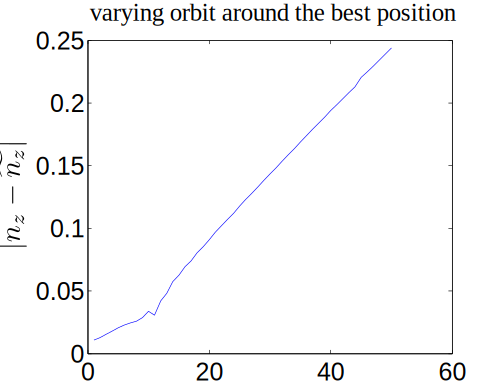
\includegraphics[width=0.7\textwidth]{figures/results/particleA/A_orbitVariation.pdf}
 \end{center}
 \caption{The difference between the theoretical $n_z$ and the measured $\widetilde{n_z}$ for the first stretch of the first measurement for particle A (seen in figure \ref{fig:particleA1})with the best asymmetry for different orbits. .}
 \label{fig:orbitVariation}
 \end{figure}
 
 
 \begin{figure}[H]
 \begin{center}
 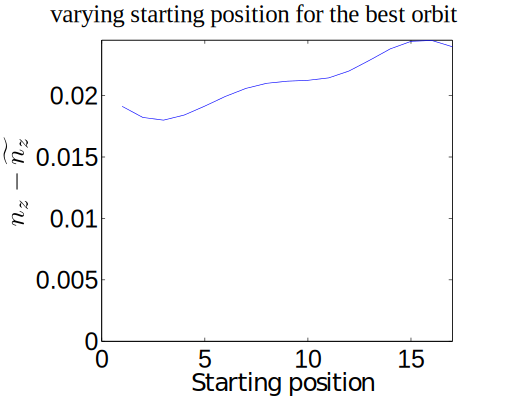
\includegraphics[width=0.7\textwidth]{figures/results/particleA/A_posVariation.pdf}
 \end{center}
 \caption{The difference between the theoretical $n_z$ and the measured $\widetilde{n_z}$ for the first stretch of the first measurement for particle A. The best orbit and best asymmetry are chosen, but different initial conditions are tested. }
 \label{fig:initVariation}
 \end{figure}